\documentclass[a4paper,12pt]{article}
\usepackage{hyperref}
\usepackage{fullpage}
\usepackage{caption}
\usepackage{subcaption}
\usepackage{url}
\usepackage{graphicx}
\usepackage{hyperref}
\usepackage{listings}
\usepackage{color}
\usepackage{listings}
\usepackage{color}
 
\definecolor{dkgreen}{rgb}{0,0.6,0}
\definecolor{gray}{rgb}{0.5,0.5,0.5}
\definecolor{mauve}{rgb}{0.58,0,0.82}
 
\lstset{ %
  language=python,                % the language of the code
  basicstyle=\footnotesize,           % the size of the fonts that are used for the code
  numbers=left,                   % where to put the line-numbers
  numberstyle=\tiny\color{gray},  % the style that is used for the line-numbers
  stepnumber=2,                   % the step between two line-numbers. If it's 1, each line 
                                  % will be numbered
  numbersep=5pt,                  % how far the line-numbers are from the code
  backgroundcolor=\color{white},      % choose the background color. You must add \usepackage{color}
  showspaces=false,               % show spaces adding particular underscores
  showstringspaces=false,         % underline spaces within strings
  showtabs=false,                 % show tabs within strings adding particular underscores
  frame=single,                   % adds a frame around the code
  rulecolor=\color{black},        % if not set, the frame-color may be changed on line-breaks within not-black text (e.g. comments (green here))
  tabsize=2,                      % sets default tabsize to 2 spaces
  captionpos=b,                   % sets the caption-position to bottom
  breaklines=true,                % sets automatic line breaking
  breakatwhitespace=false,        % sets if automatic breaks should only happen at whitespace
  title=\lstname,                   % show the filename of files included with \lstinputlisting;
                                  % also try caption instead of title
  keywordstyle=\color{blue},          % keyword style
  commentstyle=\color{dkgreen},       % comment style
  stringstyle=\color{mauve},         % string literal style
  escapeinside={\%*}{*)},            % if you want to add LaTeX within your code
  morekeywords={*,...},              % if you want to add more keywords to the set
  deletekeywords={...}              % if you want to delete keywords from the given language
}
\author{----\\ \texttt{o@c.mx}}
\title{Genome Informatics}
\bibliographystyle{plain}

\begin{document}
\maketitle
\section{QC and Assembly of the short reads using Velvet}
The paired-end short reads came in fastq file which means that the
file includes a quality score $Q$ for each base.  This score is
automatically assigned to each base by the sequencing machine and it
relates to the probability of there being a sequencing error on that
base like so: $Q = -10 \log_{10} (P)$, where $P$ is the probability of
an error which is determined by factors like how far in the read we
are, bases being sequenced and other biases introduced by the
technology.
%% The data were generated by an Illumina NGS machine so we
%% expect the quality of the reads to deteriorate towards the end of the
%% reads which is related to the fluorescent base markers and polymerase
%% used in the sequencing process.
I used FastQC
[\cite{andrews2010fastqc}] to get and plot the average quality scores
across the bases of each read.  In Figure \ref{fig:qc} we can see the
average and variation of quality scores (blue line and yellow box
respectively) across the bases for our 76-bp reads for both set of
reads. As expected, we observe a dramatic decrease in the quality as
we go along towards the end of the reads. In the last 15 bases the
quality scores go below 10 which corresponds to an uncertainty of more
that 10\% about the correctness of the base.

After this initial quality control I attempted to assemble the
paired-end short reads using Velvet, a De Bruijn graph based
assembler[\cite{zerbino2008velvet}]. Velvet, like all other De Bruijn
graph assemblers, fragments the input reads into k-mers which are
translated to nodes in the graph and then uses read information again
to connect the different k-mers.  One important concept used by Velvet in
later error correction stages is that of coverage. If we think of
reads as paths through the graph then the number of paths that a node
or k-mer appears in is the coverage of that k-mer/node. Firstly Velvet
tries to do error correction by identifying topological features of
the graph that correspond to errors, like bubbles and unconnected tips
in the graph. Then it does a removal of errors that do not correspond
to particular topological features by a straight coverage cutoff on
the basis that nodes with lower coverage probably correspond to
sequencing or other errors. During this error removal stage Velvet is
being particularly conservative about what it prunes from the graph
and delegates the responsibility to the user to choose sensible
parameters to tune that error correction which can have a big effect
on the overall produced assembly.  One of these parameter is the
coverage cutoff which is used in the straight coverage cutoff step
after the removal of bubbles and tips. By removing these low coverage
erroneous connections we get better connectivity and an easier to solve graph. However being too aggressive with the cutoff could result in losing genuine connections and misassemblies. Another parameter is the
expected coverage which biases Velvet towards taking or not some
simplification steps. For example if we have one path of a bubble with
average coverage much less than expected then Velvet is more likely to
collapse the bubble to the second path with average coverage closer to
the expected one. It is important not to choose to high or too low of
a value because that will cause Velvet to make spurious decisions
which might result in losing information or misassemblies.

For all the runs of Velvet the parameter $k$ for the k-mer size was
chosen to be $31$. I first run Velvet without any parameters to see
the node coverage distribution so I could choose sensible parameters
for expected coverage, coverage cutoff, as described in Velvet
manual. As expected, running without parameters, the assembly contains
a lot of erroneous connections (no cutoff used and Velvet does not use
one by default) and therefore we do not get contigs of significant
size which is reflected in a low N50 of 166 and a big number of nodes(940576).
The length weighted node coverage distribution for the initial run
without parameters can be seen in Figure \ref{fig:cov_dist_all}. As
expected there is a really high concentration of low coverage nodes
. I decided, based
on this initial node coverage distribution, to use a coverage cutoff
of $3.5$ because this is where the majority of the high frequency low
coverage nodes lies.  Looking at the distribution after the cutoff
value of $3.5$ (Figure \ref{fig:cov_dist_cc}), previously shadowed by
the high frequency low coverage nodes below $3.5$, the expected
coverage looks $\approx 30$.

Running Velvet again with previously selected parameters of
\verb+exp_coverage=30+ and \verb+cov_cutoff=3.5+ we get much better
results, as expected. We get an N50 of 10047, for a total number of
3600 nodes with 6468410 out of the total 14153894 used in the final
assembly. The max contig length is 57549-bp.
\begin{figure}
\centering
\begin{subfigure}{.5\textwidth}
  \centering
  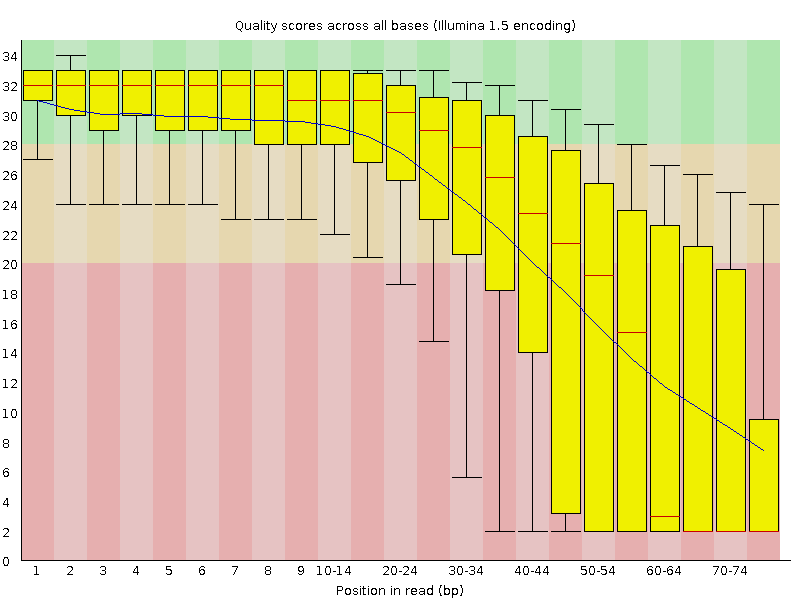
\includegraphics[width=1.\linewidth]{images/per_base_quality_r1}
  \caption{}
  \label{fig:r1_qc}
\end{subfigure}%
\begin{subfigure}{.5\textwidth}
  \centering
  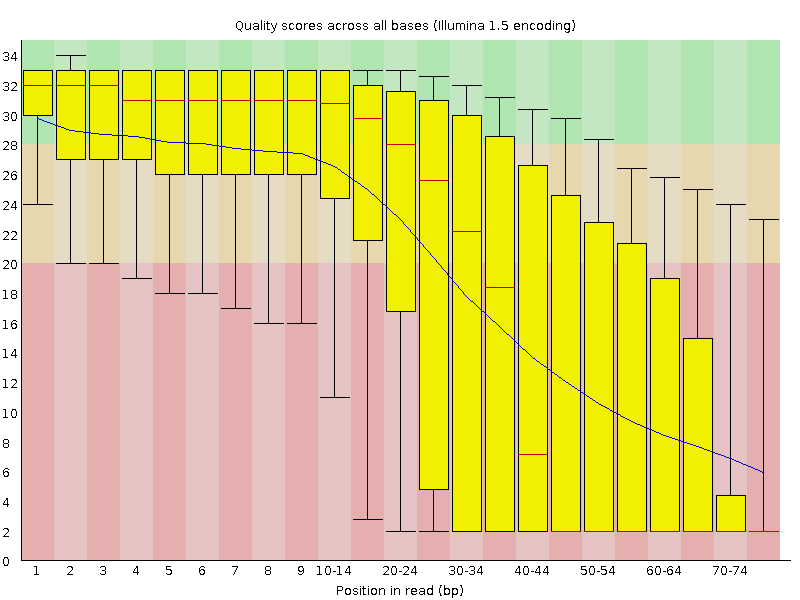
\includegraphics[width=1.\linewidth]{images/per_base_quality_r2.png}
  \caption{}
  \label{fig:r2_qc}
\end{subfigure}
\caption{
  On the left hand side a report on the quality scores across the
  bases for one end of the reads and on the right hand side the same
  for the other end of the reads. The blue line is the average quality
  score while the yellow box is the IRQ of the quality scores for that
  base.
}
\label{fig:qc}
\end{figure}

\begin{figure}
\centering
\begin{subfigure}{.5\textwidth}
  \centering
  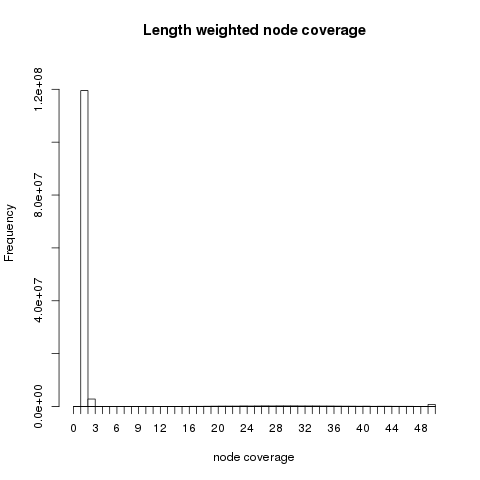
\includegraphics[width=1.\linewidth]{images/noparams_wcov}
  \caption{}
  \label{fig:cov_dist_all}
\end{subfigure}%
\begin{subfigure}{.5\textwidth}
  \centering
  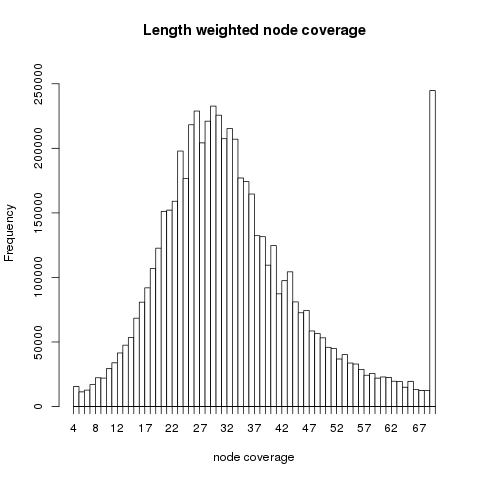
\includegraphics[width=1.\linewidth]{images/noparams_wcov_cc}
  \caption{}
  \label{fig:cov_dist_cc}
\end{subfigure}
\caption{On the left, the entire length weighted node coverage distribution. On the right, the node coverage distribution with values below 4 cut off.}
\label{fig:cov_dist}
\end{figure}

\section{Alignment of assembled contigs to closest sequenced relative}
\label{sec:alignment}
After getting the assembled contigs from the run of Velvet with
optimal parameters I programmatically probed NCBI's BLAST servers for
matches in the database of reference genomes for matches with 5 of the
largest contigs found in the \verb+contigs.fa+ file produced by
Velvet. I then selected as closest organism the organism present the
most times in the top 3 hits for the 5 contigs. This approach could
have potential problems if our contigs fall within genome regions with
highly important functions which are conserved through different
species. In that case many, even unrelated species, could produce
significant matches with our contigs. However the length of our
contigs gives us confidence that they will carry enough information to
overcome those potential problems. The organism present most times in
the top hits of the larger contigs was the SBW25 strain of the
Pseudomonas fluorescens bacterium. A manual inspection of the top hits
from the largest contigs shows that the database matches of our
contigs are all to different strains of Pseudomonas fluorescens
bacterium or other closely related species so that backs up our
findings and excludes the possibility of spurious results due to the
previously mentioned problems.

To compare the assembled contigs produced with Velvet with the genome
of its closest bacterial strain I used
MUMMER[\cite{kurtz2004versatile}] to align the contigs to the
reference genome of Pseudomonas fluorescens SBW25. The assembled
contigs cover $\approx 64\%$ of the reference genome. Of the 3600
assembled contigs, only 1163 are aligned to the reference genome. Of
those 1163 aligned contigs 659 have a single alignment to the
reference containing at least 88\% of the contig length. Overall, the
aligned contigs align on average to $2.73$ locations on the
reference with the alignments containing on average 89\% of the contig. By inspection of the mapping of query contig sequence to
the reference obtained, which includes connections between the
different alignments of the same query, the locations of the different
alignments of the same contigs are in close proximity to each
other(Figure~\ref{fig:map}). The small gaps between different alignment of the same contig may be due to local assembly errors
or local structural variation(insertions, deletions). The aligned
parts of the contigs have on average 91\% identity with their
homologous sequences in the reference.

\begin{figure}
  \centering
  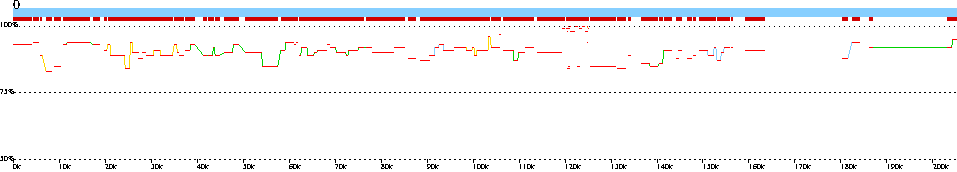
\includegraphics[scale=0.53]{images/map_region}
  \caption{Indicative region of the mapping of the aligned contigs to the reference sequence. Matches from the same contig are connected with coloured line. The vertical position of the matches(red rectangles) indicate the \% identity with their homologous sequence on the reference(indicated with the blue colour on top)}

  \label{fig:map}
\end{figure}

\section{Differences in gene content between the two species}
From the indicative region of the mapping of the contigs to the
reference region(Figure~\ref{fig:map}) and the coverage percentage
reported in the previous section it is obvious that there are multiple
gaps in the alignment of the assembled contigs to the reference. Small
gaps between different alignments of parts of the same contig could be
attributed to local assembly errors or local biological variation
(insertions/deletions). The bigger gaps could be a product of the
assembly or just genuine genetic variation between the two
strains. The main causes of misassemblies are repeated regions in the
genomes which could cause a collapse between those regions resulting
in loss of read information between. However bacteria in general do
not have big repeated regions and in particular the repeated regions
in the Pseudomonas species represent a small percentage of the entire
genome and range in sizes smaller than the insert length of our
paired-end reads. This should be enough for Velvet to take care of
ambiguities created by those short repeated regions. Moreover,
comparative studies of the different strains of the Pseudomonas
species have shown considerable differences between
them[\cite{silby2009genomic}]. These evidence point towards genuine
genetic variation for the reason for the gaps in the alignment.

To investigate the variation I looked at what genes are annotated as
being in the location of the largest gap in the reference genome,
their products, and the pathways they are involved in. The biggest gap
is of size 140076 and is located between 2050454-bp and 2190530-bp on the
reference. Pseudomonas fluorescens SBW25 has a high coding
density(88.3\%,[\cite{silby2009genomic}]) so naturally in such big of a
gap there are a lot of genes. A first search on NCBI's gene databases
returns $140$ genes in that region of the genome. I narrowed the
search down by keeping only genes that have a RefSeq status REVIEWED
or VALIDATED and also removed pseudogenes. The resulting $5$ genes are the following:
PFLU1972, PFLU1996, PFLU2009, PFLU1949, and PFLUt47. 
From those genes, the first 4 are protein coding and the last one is a tRNA
gene. PFLU1972 codes for protein DNA topoisomerase III which is
involved in DNA winding operations. It has conserved domains
related to that, specifically, TOP1Ac, TOPRIM\_TopoIA\_TopoIII, and
zf-C4\_Topoisom. These perform operations on DNA strands, like
rejoining broken phosphodiester bonds and removing negative
supercoils. With the exception of PFLU1996 which only has putative
protein product the other 3 genes are involved in biosynthesis of
different products. The protein product of PFLU2009 is threonine
synthase and has conserved domains related to threonine biosynthesis,
Thr-synth\_2 which catalyses the final step of threonine biosynthesis
and ThrC which is involved in transportation and metabolism of that
amino acid. This gene is therefore involved in the corresponding
pathways for organism-specific and conserved biosynthesis and
metabolism of amino acids and threonine.PFLU1949 codes for protein
product histidinol dehydrogenase which catalyses the final step in the
biosynthesis of another amino acid, histidine. It has the corresponding
conserved domains, Histidinol\_dh, and hisD for histidinol
dehydrogenase. Finally the tRNA gene, PFLUt47, is involved in
conserved and organism-specific pathways for aminoacyl-tRNA
biosynthesis.

\section{Methods}
Most of the code was written in Python with the use, in some places,
of appropriate BioPython modules. R was also used in some places where
it was convenient(for example to easily access and manipulate result
files created by Velvet and nucmer). The code accompanies this report (see Appendix \ref{app:src} and it is also available along with all
data, images and the code for this report \href{http://people.ds.cam.ac.uk/az325/assembly/}{here}.
The following shows the commands I used to get my results(assumes a directory structure as found in the online version of the code):
\begin{verbatim}
python scripts/preprocess.py data/reads1.fq data/reads2.fq
FastQC/fastqc -f data/reads1_val.fq data/reads2_val.fq
velveth data 31 -shortPaired -fastq data/reads.fq
velvetg data -exp_cov 30 -cov_cutoff 3.5 -ins_length 500
python scripts/blast_q.py data/contigs.fa
nucmer -maxmatch -c 100 -p data/nucmer data/sequence.fasta data/contigs.fa
show-coords -r -c -l  data/nucmer.delta > data/nucmer.coords
mapview -n 1 -f png -Ir -p data/maps data/nucmer.coords
python scripts/parse_coords.py data/nucmer.coords
\end{verbatim}

\bibliography{report}
\appendix
\label{app:src}
\section{Code}
\lstinputlisting{/home/argyris/assembly/scripts/preprocess.py}
\lstinputlisting[language=R]{/home/argyris/assembly/scripts/assembly_stats.R}
\lstinputlisting{/home/argyris/assembly/scripts/blast_q.py}
\lstinputlisting[language=R]{/home/argyris/assembly/scripts/align_stats.R}
\lstinputlisting{/home/argyris/assembly/scripts/annotations.py}
\lstinputlisting{/home/argyris/assembly/scripts/parse_coords.py}
\end{document}
